\begin{pastexam}[label={px:ncku-112-isec-ds-05}]{成大智慧資安學程 112 學年度 第 5 題}
（問答）

(10\%) Landscapes in films are often computer generated. Ever wondered how they do it? Here is an
algorithmic drawing example. Draw enough repeating patterns until you can tell what it is. Start by
drawing a single straight vertical line as below

\begin{center}
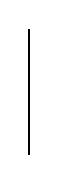
\begin{tikzpicture}
\draw[thick] (0,0)--(0,1.6);
\end{tikzpicture}
\end{center}

Then execute Draw( ) from this vertical line until you can show how the algorithmic drawing works.

\begin{center}
\fbox{\begin{minipage}{0.9\textwidth}\sffamily
Draw( )\\
\{\\[2pt]
{\footnotesize
\hspace*{1.5em}Draw 3 shorter lines at an angle in the top two-thirds of the line on its left side.\\[2pt]
\hspace*{1.5em}Draw 3 shorter lines at an angle in the top two-thirds of the line on its right side.\\[2pt]
\hspace*{1.5em}Choose a new existing line and Draw( ) from that line again\\[2pt]}
\}
\end{minipage}}
\end{center}
\end{pastexam}

\begin{pastsoln}
答案：畫出來的是一棵\textbf{樹}（像松樹、杉樹那樣的針葉樹，枝條一層一層分叉）。

\textbf{讀法}。 Draw( ) 作用在「一條線」上：在這條線靠末端的三分之二段上取三個點，每個點往左、往右
各斜斜長出一條比較短的線，一共六條新線；然後挑一條已經存在的線，對它再做一次 Draw( )。 原題沒有
規定角度、長度和分叉點的確切位置，下面取：分叉點平均分布在上方三分之二段（離起點 $1/3$、$5/9$、
$7/9$ 處），新線和原來的線夾 $40^\circ$、往線的末端方向斜，長度依序是原線的 $0.5$、$0.4$、$0.3$
倍（越靠末端越短）。 角度和長度換成別的值，畫出來仍然是樹，只是枝條的疏密不同。

\textbf{執行過程}。 每一輪把上一輪新長出的線都做一次 Draw( )（等於「挑一條線」挑完一整輪）：
\begin{center}
\begin{tikzpicture}[x=0.85cm,y=0.85cm,line cap=round]
\begin{scope}[xshift=0cm]
\draw[line width=1.2pt] (0.00,0.00)--(0.00,3.00);
\node[font=\small] at (0,-0.4) {開始};
\end{scope}
\begin{scope}[xshift=3.4cm]
\draw[line width=1.2pt] (0.00,0.00)--(0.00,3.00);
\draw[line width=0.8pt] (0.00,1.00)--(-0.96,2.15) (0.00,1.00)--(0.96,2.15) (0.00,1.67)--(-0.77,2.59) (0.00,1.67)--(0.77,2.59) (0.00,2.33)--(-0.58,3.02) (0.00,2.33)--(0.58,3.02);
\node[font=\small] at (0,-0.4) {第 1 輪};
\end{scope}
\begin{scope}[xshift=6.8cm]
\draw[line width=1.2pt] (0.00,0.00)--(0.00,3.00);
\draw[line width=0.8pt] (0.00,1.00)--(-0.96,2.15) (0.00,1.00)--(0.96,2.15) (0.00,1.67)--(-0.77,2.59) (0.00,1.67)--(0.77,2.59) (0.00,2.33)--(-0.58,3.02) (0.00,2.33)--(0.58,3.02);
\draw[line width=0.5pt] (-0.32,1.38)--(-1.06,1.51) (-0.32,1.38)--(-0.32,2.13) (-0.54,1.64)--(-1.13,1.74) (-0.54,1.64)--(-0.54,2.24) (-0.75,1.89)--(-1.19,1.97) (-0.75,1.89)--(-0.75,2.34) (0.32,1.38)--(0.32,2.13) (0.32,1.38)--(1.06,1.51) (0.54,1.64)--(0.54,2.24) (0.54,1.64)--(1.13,1.74) (0.75,1.89)--(0.75,2.34) (0.75,1.89)--(1.19,1.97) (-0.26,1.97)--(-0.85,2.08) (-0.26,1.97)--(-0.26,2.57) (-0.43,2.18)--(-0.90,2.26) (-0.43,2.18)--(-0.43,2.66) (-0.60,2.38)--(-0.95,2.44) (-0.60,2.38)--(-0.60,2.74) (0.26,1.97)--(0.26,2.57) (0.26,1.97)--(0.85,2.08) (0.43,2.18)--(0.43,2.66) (0.43,2.18)--(0.90,2.26) (0.60,2.38)--(0.60,2.74) (0.60,2.38)--(0.95,2.44) (-0.19,2.56)--(-0.64,2.64) (-0.19,2.56)--(-0.19,3.01) (-0.32,2.72)--(-0.68,2.78) (-0.32,2.72)--(-0.32,3.08) (-0.45,2.87)--(-0.72,2.92) (-0.45,2.87)--(-0.45,3.14) (0.19,2.56)--(0.19,3.01) (0.19,2.56)--(0.64,2.64) (0.32,2.72)--(0.32,3.08) (0.32,2.72)--(0.68,2.78) (0.45,2.87)--(0.45,3.14) (0.45,2.87)--(0.72,2.92);
\node[font=\small] at (0,-0.4) {第 2 輪};
\end{scope}
\begin{scope}[xshift=10.2cm]
\draw[line width=1.2pt] (0.00,0.00)--(0.00,3.00);
\draw[line width=0.8pt] (0.00,1.00)--(-0.96,2.15) (0.00,1.00)--(0.96,2.15) (0.00,1.67)--(-0.77,2.59) (0.00,1.67)--(0.77,2.59) (0.00,2.33)--(-0.58,3.02) (0.00,2.33)--(0.58,3.02);
\draw[line width=0.5pt] (-0.32,1.38)--(-1.06,1.51) (-0.32,1.38)--(-0.32,2.13) (-0.54,1.64)--(-1.13,1.74) (-0.54,1.64)--(-0.54,2.24) (-0.75,1.89)--(-1.19,1.97) (-0.75,1.89)--(-0.75,2.34) (0.32,1.38)--(0.32,2.13) (0.32,1.38)--(1.06,1.51) (0.54,1.64)--(0.54,2.24) (0.54,1.64)--(1.13,1.74) (0.75,1.89)--(0.75,2.34) (0.75,1.89)--(1.19,1.97) (-0.26,1.97)--(-0.85,2.08) (-0.26,1.97)--(-0.26,2.57) (-0.43,2.18)--(-0.90,2.26) (-0.43,2.18)--(-0.43,2.66) (-0.60,2.38)--(-0.95,2.44) (-0.60,2.38)--(-0.60,2.74) (0.26,1.97)--(0.26,2.57) (0.26,1.97)--(0.85,2.08) (0.43,2.18)--(0.43,2.66) (0.43,2.18)--(0.90,2.26) (0.60,2.38)--(0.60,2.74) (0.60,2.38)--(0.95,2.44) (-0.19,2.56)--(-0.64,2.64) (-0.19,2.56)--(-0.19,3.01) (-0.32,2.72)--(-0.68,2.78) (-0.32,2.72)--(-0.32,3.08) (-0.45,2.87)--(-0.72,2.92) (-0.45,2.87)--(-0.45,3.14) (0.19,2.56)--(0.19,3.01) (0.19,2.56)--(0.64,2.64) (0.32,2.72)--(0.32,3.08) (0.32,2.72)--(0.68,2.78) (0.45,2.87)--(0.45,3.14) (0.45,2.87)--(0.72,2.92);
\draw[line width=0.3pt] (-0.57,1.43)--(-0.89,1.24) (-0.57,1.43)--(-0.81,1.71) (-0.73,1.46)--(-0.99,1.31) (-0.73,1.46)--(-0.92,1.69) (-0.90,1.48)--(-1.09,1.37) (-0.90,1.48)--(-1.04,1.66) (-0.32,1.63)--(-0.56,1.92) (-0.32,1.63)--(-0.08,1.92) (-0.32,1.80)--(-0.51,2.03) (-0.32,1.80)--(-0.13,2.03) (-0.32,1.97)--(-0.47,2.14) (-0.32,1.97)--(-0.18,2.14) (-0.73,1.67)--(-0.99,1.52) (-0.73,1.67)--(-0.93,1.90) (-0.86,1.70)--(-1.07,1.58) (-0.86,1.70)--(-1.02,1.88) (-1.00,1.72)--(-1.15,1.63) (-1.00,1.72)--(-1.11,1.86) (-0.54,1.84)--(-0.73,2.07) (-0.54,1.84)--(-0.34,2.07) (-0.54,1.97)--(-0.69,2.16) (-0.54,1.97)--(-0.38,2.16) (-0.54,2.11)--(-0.65,2.24) (-0.54,2.11)--(-0.42,2.24) (-0.90,1.92)--(-1.09,1.81) (-0.90,1.92)--(-1.04,2.09) (-1.00,1.94)--(-1.15,1.85) (-1.00,1.94)--(-1.11,2.08) (-1.09,1.95)--(-1.21,1.89) (-1.09,1.95)--(-1.18,2.06) (-0.75,2.04)--(-0.89,2.22) (-0.75,2.04)--(-0.61,2.22) (-0.75,2.14)--(-0.87,2.28) (-0.75,2.14)--(-0.63,2.28) (-0.75,2.24)--(-0.84,2.35) (-0.75,2.24)--(-0.66,2.35) (0.32,1.63)--(0.08,1.92) (0.32,1.63)--(0.56,1.92) (0.32,1.80)--(0.13,2.03) (0.32,1.80)--(0.51,2.03) (0.32,1.97)--(0.18,2.14) (0.32,1.97)--(0.47,2.14) (0.57,1.43)--(0.81,1.71) (0.57,1.43)--(0.89,1.24) (0.73,1.46)--(0.92,1.69) (0.73,1.46)--(0.99,1.31) (0.90,1.48)--(1.04,1.66) (0.90,1.48)--(1.09,1.37) (0.54,1.84)--(0.34,2.07) (0.54,1.84)--(0.73,2.07) (0.54,1.97)--(0.38,2.16) (0.54,1.97)--(0.69,2.16) (0.54,2.11)--(0.42,2.24) (0.54,2.11)--(0.65,2.24) (0.73,1.67)--(0.93,1.90) (0.73,1.67)--(0.99,1.52) (0.86,1.70)--(1.02,1.88) (0.86,1.70)--(1.07,1.58) (1.00,1.72)--(1.11,1.86) (1.00,1.72)--(1.15,1.63) (0.75,2.04)--(0.61,2.22) (0.75,2.04)--(0.89,2.22) (0.75,2.14)--(0.63,2.28) (0.75,2.14)--(0.87,2.28) (0.75,2.24)--(0.66,2.35) (0.75,2.24)--(0.84,2.35) (0.90,1.92)--(1.04,2.09) (0.90,1.92)--(1.09,1.81) (1.00,1.94)--(1.11,2.08) (1.00,1.94)--(1.15,1.85) (1.09,1.95)--(1.18,2.06) (1.09,1.95)--(1.21,1.89) (-0.45,2.01)--(-0.71,1.86) (-0.45,2.01)--(-0.65,2.24) (-0.59,2.03)--(-0.79,1.91) (-0.59,2.03)--(-0.74,2.21) (-0.72,2.05)--(-0.87,1.96) (-0.72,2.05)--(-0.83,2.19) (-0.26,2.17)--(-0.45,2.40) (-0.26,2.17)--(-0.06,2.40) (-0.26,2.31)--(-0.41,2.49) (-0.26,2.31)--(-0.10,2.49) (-0.26,2.44)--(-0.37,2.58) (-0.26,2.44)--(-0.14,2.58) (-0.59,2.21)--(-0.79,2.09) (-0.59,2.21)--(-0.74,2.39) (-0.69,2.22)--(-0.86,2.13) (-0.69,2.22)--(-0.81,2.37) (-0.80,2.24)--(-0.92,2.17) (-0.80,2.24)--(-0.89,2.35) (-0.43,2.34)--(-0.58,2.52) (-0.43,2.34)--(-0.27,2.52) (-0.43,2.44)--(-0.55,2.59) (-0.43,2.44)--(-0.31,2.59) (-0.43,2.55)--(-0.52,2.66) (-0.43,2.55)--(-0.34,2.66) (-0.72,2.40)--(-0.87,2.31) (-0.72,2.40)--(-0.83,2.54) (-0.80,2.42)--(-0.92,2.34) (-0.80,2.42)--(-0.89,2.53) (-0.88,2.43)--(-0.97,2.38) (-0.88,2.43)--(-0.95,2.51) (-0.60,2.50)--(-0.72,2.64) (-0.60,2.50)--(-0.48,2.64) (-0.60,2.58)--(-0.69,2.69) (-0.60,2.58)--(-0.51,2.69) (-0.60,2.66)--(-0.67,2.74) (-0.60,2.66)--(-0.53,2.74) (0.26,2.17)--(0.06,2.40) (0.26,2.17)--(0.45,2.40) (0.26,2.31)--(0.10,2.49) (0.26,2.31)--(0.41,2.49) (0.26,2.44)--(0.14,2.58) (0.26,2.44)--(0.37,2.58) (0.45,2.01)--(0.65,2.24) (0.45,2.01)--(0.71,1.86) (0.59,2.03)--(0.74,2.21) (0.59,2.03)--(0.79,1.91) (0.72,2.05)--(0.83,2.19) (0.72,2.05)--(0.87,1.96) (0.43,2.34)--(0.27,2.52) (0.43,2.34)--(0.58,2.52) (0.43,2.44)--(0.31,2.59) (0.43,2.44)--(0.55,2.59) (0.43,2.55)--(0.34,2.66) (0.43,2.55)--(0.52,2.66) (0.59,2.21)--(0.74,2.39) (0.59,2.21)--(0.79,2.09) (0.69,2.22)--(0.81,2.37) (0.69,2.22)--(0.86,2.13) (0.80,2.24)--(0.89,2.35) (0.80,2.24)--(0.92,2.17) (0.60,2.50)--(0.48,2.64) (0.60,2.50)--(0.72,2.64) (0.60,2.58)--(0.51,2.69) (0.60,2.58)--(0.69,2.69) (0.60,2.66)--(0.53,2.74) (0.60,2.66)--(0.67,2.74) (0.72,2.40)--(0.83,2.54) (0.72,2.40)--(0.87,2.31) (0.80,2.42)--(0.89,2.53) (0.80,2.42)--(0.92,2.34) (0.88,2.43)--(0.95,2.51) (0.88,2.43)--(0.97,2.38) (-0.34,2.59)--(-0.54,2.48) (-0.34,2.59)--(-0.49,2.76) (-0.44,2.61)--(-0.59,2.52) (-0.44,2.61)--(-0.55,2.74) (-0.54,2.62)--(-0.65,2.56) (-0.54,2.62)--(-0.62,2.73) (-0.19,2.71)--(-0.34,2.89) (-0.19,2.71)--(-0.05,2.89) (-0.19,2.81)--(-0.31,2.95) (-0.19,2.81)--(-0.08,2.95) (-0.19,2.91)--(-0.28,3.02) (-0.19,2.91)--(-0.11,3.02) (-0.44,2.74)--(-0.60,2.65) (-0.44,2.74)--(-0.56,2.88) (-0.52,2.75)--(-0.64,2.68) (-0.52,2.75)--(-0.61,2.86) (-0.60,2.76)--(-0.69,2.71) (-0.60,2.76)--(-0.67,2.85) (-0.32,2.84)--(-0.44,2.97) (-0.32,2.84)--(-0.21,2.97) (-0.32,2.92)--(-0.41,3.03) (-0.32,2.92)--(-0.23,3.03) (-0.32,3.00)--(-0.39,3.08) (-0.32,3.00)--(-0.25,3.08) (-0.54,2.89)--(-0.66,2.82) (-0.54,2.89)--(-0.63,2.99) (-0.60,2.90)--(-0.69,2.84) (-0.60,2.90)--(-0.67,2.98) (-0.66,2.91)--(-0.73,2.87) (-0.66,2.91)--(-0.71,2.97) (-0.45,2.96)--(-0.54,3.06) (-0.45,2.96)--(-0.36,3.06) (-0.45,3.02)--(-0.52,3.10) (-0.45,3.02)--(-0.38,3.10) (-0.45,3.08)--(-0.50,3.14) (-0.45,3.08)--(-0.40,3.14) (0.19,2.71)--(0.05,2.89) (0.19,2.71)--(0.34,2.89) (0.19,2.81)--(0.08,2.95) (0.19,2.81)--(0.31,2.95) (0.19,2.91)--(0.11,3.02) (0.19,2.91)--(0.28,3.02) (0.34,2.59)--(0.49,2.76) (0.34,2.59)--(0.54,2.48) (0.44,2.61)--(0.55,2.74) (0.44,2.61)--(0.59,2.52) (0.54,2.62)--(0.62,2.73) (0.54,2.62)--(0.65,2.56) (0.32,2.84)--(0.21,2.97) (0.32,2.84)--(0.44,2.97) (0.32,2.92)--(0.23,3.03) (0.32,2.92)--(0.41,3.03) (0.32,3.00)--(0.25,3.08) (0.32,3.00)--(0.39,3.08) (0.44,2.74)--(0.56,2.88) (0.44,2.74)--(0.60,2.65) (0.52,2.75)--(0.61,2.86) (0.52,2.75)--(0.64,2.68) (0.60,2.76)--(0.67,2.85) (0.60,2.76)--(0.69,2.71) (0.45,2.96)--(0.36,3.06) (0.45,2.96)--(0.54,3.06) (0.45,3.02)--(0.38,3.10) (0.45,3.02)--(0.52,3.10) (0.45,3.08)--(0.40,3.14) (0.45,3.08)--(0.50,3.14) (0.54,2.89)--(0.63,2.99) (0.54,2.89)--(0.66,2.82) (0.60,2.90)--(0.67,2.98) (0.60,2.90)--(0.69,2.84) (0.66,2.91)--(0.71,2.97) (0.66,2.91)--(0.73,2.87);
\node[font=\small] at (0,-0.4) {第 3 輪};
\end{scope}\end{tikzpicture}
\end{center}
\begin{itemize}
\item 開始：只有一條直線，就是樹幹。
\item 第 1 輪：樹幹的上方三分之二長出左右各三條枝，下面的枝長、上面的枝短，輪廓已經是三角形的樹冠。
\item 第 2 輪：六條枝各自又長出六條小枝，每條枝都變成和整棵樹相似的小樹。
\item 第 3 輪：再細一層，整體看起來就是一棵枝葉茂密的樹。
\end{itemize}
共做了 $k$ 輪時，第 $j$ 輪新增 $6^j$ 條線，總共 $1 + 6 + 6^2 + \cdots + 6^k = (6^{k+1} - 1)/5$
條；上圖四格分別是 $1$、$7$、$43$、$259$ 條。 每一條線都和整棵樹的形狀相似（局部和整體相似），
這種圖形叫碎形（fractal），電影裡的樹林、山脈常用這類遞迴規則產生。

\textbf{和資料結構的關係}。 Draw( ) 是一個遞迴程序：每次呼叫產生六條新線，再對新線呼叫自己，
呼叫關係是一棵每個節點有六個子節點的樹（6 元樹），第 $j$ 層有 $6^j$ 個呼叫。 「挑一條已經存在
的線」如果用佇列存待處理的線（先進先出），就是上面一輪一輪長的順序，相當於對這棵呼叫樹做層序走訪；
如果直接遞迴呼叫（系統堆疊，後進先出），會先把一條枝畫到最細才回頭畫別的枝，相當於深度優先
（資結書第~6.4~節、第~7.3~節）。 兩種順序畫完的圖一樣。

原題的 Draw( ) 沒有\textbf{終止條件}，照字面會無窮遞迴。 實際寫程式時要加一個基本情形，例如
「線短於某個長度（或遞迴深度達到 $k$）就不再分叉，直接返回」。
\end{pastsoln}
